\documentclass[
  shortnames]{jss}

%% recommended packages
\usepackage{orcidlink,thumbpdf,lmodern}

\usepackage[utf8]{inputenc}

\author{
Gilberto Camara~\orcidlink{0000-0002-3681-487X}\\Nat Inst for Space Research\\
Brazil \And Renato Assunção~\orcidlink{0000-0001-7442-9166}\\Federal Univ of Minas Gerais\\
Brazil \And Rolf Simoes~\orcidlink{0000-0003-0953-4132}\\Nat Inst for Space Research\\
Brazil \AND Alexandre Carvalho~\orcidlink{0000-0001-8762-5465}\\Inst Applied Economic Research\\
Brazil \And Felipe Souza~\orcidlink{0000-XXXXX}\\Nat Inst for Space Research\\
Brazil \And Pedro R. Andrade~\orcidlink{0000-0001-8675-4046}\\Nat Inst for Space Research\\
Brazil
}
\title{Bayesian inference for post-processing of remote sensing image classification}

\Plainauthor{Gilberto Camara, Renato Assunção, Rolf Simoes, Alexandre Carvalho, Felipe Souza, Pedro R. Andrade}
\Plaintitle{Bayesian smoothing for image classification}
\Shorttitle{Bayesian smoothing for image classification}


\Abstract{
A key component of remote sensing image analysis is image classification, which aims to categorize the pixels in an image into different classes using machine learning methods. The result of machine learning classifiers is a set of class probabilities for each pixel. These class probabilities are the input to post-processing techniques that aim to improve on the machine learning results. This paper introduces a new post-processing algorithm that uses an Empirical Bayes approach. To simulate the impact of discontinuity between land classes, we use non-isotropic neighborhood definitions. Our method allows the inclusion of expert knowledge to enhance the consistency of the resulting map. The method has been validated for large-scale data analysis in connection with a time-first, space-based approach and is available in the R package \pkg{bayesEO}.
}

\Keywords{Bayesian smoothing, image classification, machine learning, \proglang{R}}
\Plainkeywords{Bayesian smoothing, image classification, machine learning, R}

%% publication information
%% \Volume{50}
%% \Issue{9}
%% \Month{June}
%% \Year{2012}
%% \Submitdate{}
%% \Acceptdate{2012-06-04}

\Address{
    Gilberto Camara\\
    Nat Inst for Space Research\\
Brazil\\
    Avenida dos Astronautas, 1758\\
12227-001 Sao Jose dos Campos, Brazil\\
  E-mail: \email{gilberto.camara```inpe.br}\\
  
            }


% tightlist command for lists without linebreak
\providecommand{\tightlist}{%
  \setlength{\itemsep}{0pt}\setlength{\parskip}{0pt}}

% From pandoc table feature
\usepackage{longtable,booktabs,array}
\usepackage{calc} % for calculating minipage widths
% Correct order of tables after \paragraph or \subparagraph
\usepackage{etoolbox}
\makeatletter
\patchcmd\longtable{\par}{\if@noskipsec\mbox{}\fi\par}{}{}
\makeatother
% Allow footnotes in longtable head/foot
\IfFileExists{footnotehyper.sty}{\usepackage{footnotehyper}}{\usepackage{footnote}}
\makesavenoteenv{longtable}



\usepackage{amsmath} \usepackage{microtype} \usepackage{graphicx} \usepackage{booktabs} \usepackage{float} \usepackage{flafter} \usepackage{placeins} \usepackage[all,defaultlines=3]{nowidow} \usepackage[T1]{fontenc} \usepackage[adobe-utopia]{mathdesign} \renewcommand*\ttdefault{txtt}

\begin{document}



\newpage

\section{Introduction}\label{introduction}

The use of remote sensing images is essential for environmental management. Satellite images have a wide range of applications, including measuring changes in land cover and assessing agriculture and natural habitats. Satellite measurements are the only viable mean to repeatedely survey vast regions, such tropical forests and the polar regions. Remote sensing data plays a critical role in protecting the environment by supplying essential information to policymakers and conservationists.

Image classification is an key component of remote sensing image analysis. The goal of this task is to categorize the pixels in an image into different classes based on their spectral characteristics, spatial patterns, or other relevant features. Researchers employ machine learning methods like random forests \citep{Belgiu2016} and deep learning \citep{Ma2019} in image classification. The result of machine learning classifiers is a set of class probabilities for each pixel, organised in matrices that are identical in size to the original image. Each matrix provides the probability of a pixel's class membership. These matrices are the input to post-processing techniques that aim to improve on the machine learning results. Post-processing leads to improved accuracy and better interpretability of the final output by reducing errors and minimizing noise \citep{Schindler2012}.

Due to the complexity of remote sensing data, classification algorithms can introduce noise or produce outliers. Spectral responses of ground targets have large variability. Pixels in medium-resolution satellite images, like Landsat or Sentinel-2, often have mixed spectral responses from different land cover types. For these reasons, classifiers produce results that include misclassified pixels, especially in the boundaries between two homogenous ground objects which have different spectral responses. Post-processing methods need to be able to detect and correct such errors.

The fragment of a Sentinel-2 image from in Rondonia, Brazil, shown in Figure \ref{fig:roim}, illustrates why post-processing is required for image classification. In the image, one can see the distinction between green forest areas and deforested areas depicted in shades of orange and brown. The border pixels between green forest areas and brown bare soil have mixed responses. In many cases, such mixed pixels will be labelled as a third class which does not occur in this area. Thus, these border pixels are prone to misclassification, which needs to be corrected using suitable post-processing methods.

\begin{CodeChunk}
\begin{figure}[h]

{\centering 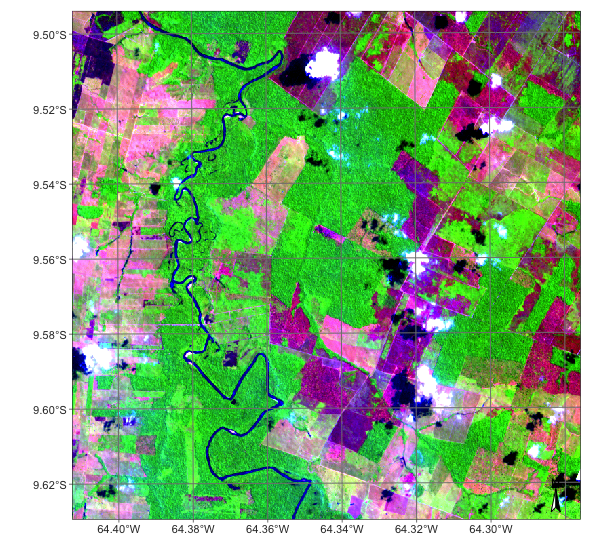
\includegraphics[width=0.8\linewidth]{images/rgb_image} 

}

\caption[Detail of Sentinel-2 image in the Amazon forest]{Detail of Sentinel-2 image in the Amazon forest.}\label{fig:roim}
\end{figure}
\end{CodeChunk}

Image classification post-processing methods include Gaussian, semi-global, bilateral, and edge-aware filtering \citep{Schindler2012}, modal filters \citep{Ghimire2010}, and co-occurrence matrices \citep{Huang2014}. All these methods have limitations to deal with boundary pixels. Both Gaussian and semi-global smoothing methods assume that each class has a uniform local variance value. These approaches assume probabilities change gradually within a window centred on each pixel, which is not the case for border pixels. As a result, these methods blur the crisp boundaries that separate homogenous regions in the image. Gaussian and semi-global smoothing techniques are ineffective in addressing the problem of mixed pixels at object boundaries \citep{Huang2014}. Bilateral smoothing uses two global parameters to maintain boundary shapes \citep{Schindler2012}. The algorithm assumes that the spatial distribution of the class probabilities is isotropic in a pixel's neighbourhood. As we argue in this paper, such an assumption does not hold for border pixels. Hence, there is a need for post-processing methods that can handle situations involving mixed pixels and anisotropic neighborhoods.

The paper introduces a new post-processing algorithm for remote sensing image classification using an Empirical Bayes approach. The algorithm is available in the \proglang{R} package \pkg{bayesEO}. To simulate the impact of discontinuity between land classes, we use non-isotropic neighborhood definitions. Our method allows the inclusion of expert knowledge to enhance the consistency of the resulting map. The \pkg{bayesEO} package can be combined with \pkg{sits}, an end-to-end toolkit for land use and land cover classification using big Earth observation data developed by the authors \citep{Simoes2021}.

Our package adds to other \proglang{R} libraries focused on the spatial data analysis, including \pkg{spdep} \citep{Bivand2023} and \pkg{rgeoda} \citep{Li2022}. \pkg{CARBayes} \citep{Lee2013} implements Bayesian models for spatial areal units. For image processing analysis, \pkg{terra} \citep{Hijmans2023} provides supervised classification with decision trees, while \pkg{stars} \citep{Bivand2023} includes functions for linear regression and random forest classification. For post-processing of machine learning image classification, \pkg{sits} also uses the method described in this paper. As far as we know, no current \proglang{R} package supports post-processing of image classification of remote sensing images. For this reason, we consider \pkg{bayesEO} to be a useful addition to the facilities available in \proglang{R} for remote sensing image processing.

\newpage

\section{Methods}\label{methods}

\subsection{The land classification problem}\label{the-land-classification-problem}

In land classification, we deal with categorical data, with each category corresponding to a different land type (e.g., forest, grassland, wetland, crop). Land classification aims to subdivide the space into discrete areas, each associated with a distinct type of land use or cover. Borders between different land classes usually represent sharp transitions. Formally, the land classification problem can be expressed as follows. Given a set of \(n\) spatial locations or pixels \(S = \{ \mathbf{s}_1, \ldots, \mathbf{s}_n \}\), each with an associated \(d\)-dimensional feature vector \(\mathbf{x}_1, \ldots, \mathbf{x}_s\) with values in \(\mathcal{X} \subset \mathbb{R}^m\) and a set of \(m\) land classes \(K = \{ 1, ..., m \}\), we seek a classification function \(f\) such that

\begin{align}
f\colon S \times \mathcal{X} & \longrightarrow K \nonumber \\
(\mathbf{s}_i, \mathbf{x}_i) & \longmapsto (p_{i,1}, \ldots, p_{i,m}) 
\label{eq:classificationf}
\end{align}

with \(0 \leq p_{i,k} \leq 1\) and \(\sum_k p_{i,k} = 1 \forall i = 1, \ldots, n\). The value \(p_{i,k}\) is interpreted as the probability that the \(i\)-th pixel belongs to the \(k\)-th class. The class assigned to the pixel is determined by the highest probability among the available options.

For pixel-based classification methods the spatial \(\mathbf{s}_i\) dimension is not explicitly used by the classification function \(f\). The reason is that \(f\) is obtained from a training dataset \(T = \{ \mathbf{s}_{t_1}, \ldots, \mathbf{s}_{t_s} \} \subset S\) with \(s \ll n\). Each element \(\mathbf{s}_{t_i} \in T\) is coupled with one single label \(k_{t_i} \in K\) representing the class to which it belongs, even when the pixel has mixed classes on the ground. This training dataset is also called the \textit{ground truth} dataset. Usually, it is composed of non-contiguous locations and therefore, there is no spatial neighborhood context available to train \(f\). The only resource to fit \(f\) are the true labels features \(\mathbf{x}\) measured at each location in the training dataset \(T\).

\begin{CodeChunk}
\begin{figure}[!h]

{\centering 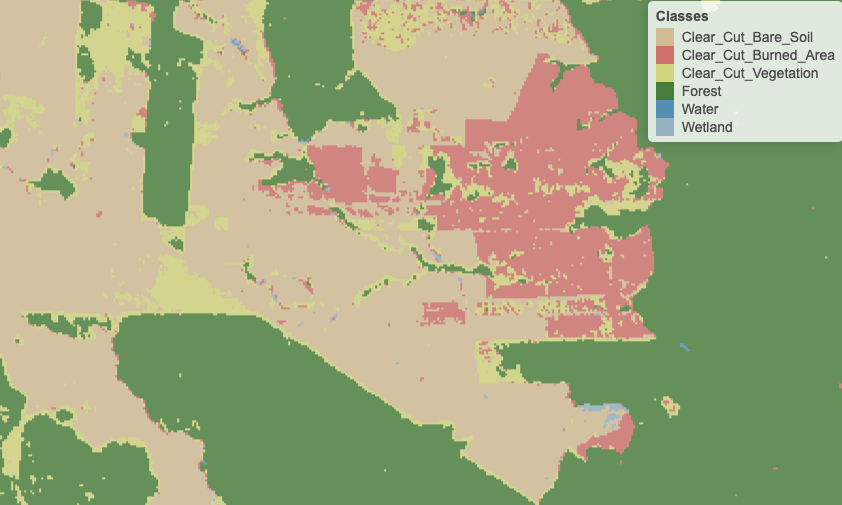
\includegraphics[width=0.7\linewidth]{images/map_no_smooth_v2} 

}

\caption[Detail of labelled map produced by pixel-based random forest without smoothing (source]{Detail of labelled map produced by pixel-based random forest without smoothing (source: authors)}\label{fig:mapnosmooth}
\end{figure}
\end{CodeChunk}

The main idea behind our post-processing method is that a pixel-based classification should take into account its neighborhood pixels. Consider Figure \ref{fig:mapnosmooth} which shows a class assignment produced by a random forest algorithm on a image time series in a subset of the area shown in Figure \ref{fig:roim}. The image time series has been classified using the \proglang{R} package \pkg{sits}\citep{Simoes2021}.

The classified map has been produced by taking, for each pixel, the class of higher probability produced by the algorithm. The resulting map has many noisy areas with a high spatial variability of class assignments. This happens more frequently in two cases: (a) small clusters of pixels of one class inside a larger area of a different class; (b) transition zones between classes. In general, images of heterogeneous landscapes with high spatial variability have many mixed pixels, whose spectral response combines different types of land cover in a single ground resolved cell. For example, many pixels in the border between areas of classes \code{Forest} and \code{Clear_Cut_Bare_Soil} are wrongly assigned to the \code{Clear_Cut_Vegetation} class. This wrong assignment occurs because these pixels have a mixed response. Inside the ground cell captured by the sensor as a single pixel value, there are both trees and bare soil areas. Such results are undesirable and need to be corrected by post-processing.

To maintain consistency and coherence in our class representations, we should minimise small variations or misclassifications. We incorporate spatial coherence as a post-processing step to accomplish this. The probabilities associated with each pixel will change based on statistical inference, which depends on the values for each neighbourhood. Using the recalculated probabilities for each pixel, we get a better version of the final classified map.

\begin{CodeChunk}
\begin{figure}[!h]

{\centering 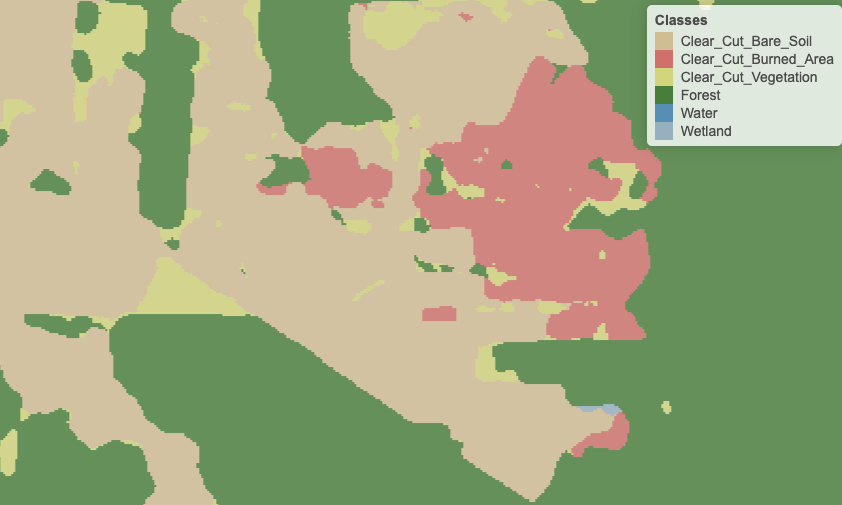
\includegraphics[width=0.7\linewidth]{images/map_smooth_v2} 

}

\caption[Detail of labelled map produced by pixel-based random forest after smoothing (source]{Detail of labelled map produced by pixel-based random forest after smoothing (source: authors)}\label{fig:mapsmooth}
\end{figure}
\end{CodeChunk}

Consider Figure \ref{fig:mapsmooth}, which is the result of Bayesian smoothing on the random forest algorithm outcomes. The noisy border pixels between two large areas of the same class have been removed. We have also removed small clusters of pixels belonging to one class inside larger areas of other classes. The outcome is a more uniform map, like the ones created through visual interpretation or object-based analysis. Details like narrow vegetation corridors or small forest roads might be missing in the smoothed image. However, the improved spatial consistency of the final map compensates for such losses, due to the removal of misclassified pixels that have mixed spectral responses.

\subsection{A Bayesian approach to smooth image classification probabilities}\label{a-bayesian-approach-to-smooth-image-classification-probabilities}

We propose a Bayesian approach for post-processing of pixel probabilities. The classification algorithm outputs the feature-based probability estimates \((p_{i,1}, \ldots, p_{i,m})\) from (\ref{eq:classificationf}). Let \(\pi_{i,k} \geq 0\) be the prior probability of the \(i\)-th pixel belonging to class \(k \in \{1, \ldots, m\}\). We convert the observed values to the logit scale to allow for less modelling restrictions.

We assume that the logit of the prior probability of the pixels \(i\) associated to class \(k\) is described by a Gaussian distribution function

\begin{equation} 
x_{i,k} = \log\left( \frac{\pi_{i,k}}{1-\pi_{i,k}} \right) \sim N(m_{i,k}, s^2_{i,k}) 
\end{equation}

where \(m_{i,k}\) represents the mean value and \(s^2_{i,k}\) the class variance. We express the likelihood as a conditional Gaussian distribution of the logit \(x_{i,k}\) of the observed values \(p_{i,k}\) over \(\mu_{i,k}\):
\begin{equation}
(x_{i,k} | \mu_{i,k}) = \log(p_{i,k}/(1-p_{i,k})) \sim N(\mu_{i,k}, \sigma^2). 
\end{equation}

In the above equation, \(\mu_{i,k}\) is the posterior expected mean of the logit probability associated to the \(i-th\) pixel. The variance \(\sigma^2_{k}\) will be estimated based on user expertise and taken as a hyperparameter to control the smoothness of the resulting estimate. The standard Bayesian updating \citep{Gelman2014} leads to the posterior distribution

\begin{equation}
(\mu_{i,k} | x_{i,k}) \sim \sum N\left(  \frac{m_{i,k} \sigma^2_{k} +
    x_{i,k} s^2_{i,k}}{ \sigma^2_{k} +s^2_{i,k}} , \left( \frac{1}{\sigma_k^2} + \frac{1}{s^2_{i,k}} \right)^{-1} \right) 
\label{eq:BayesUpdate}
\end{equation}

The estimate calculates the posterior distributions for each class; the pixel will be assigned to the class with higher posterior mean. The posterior mean is a weighted average between the observed logit value \(x_{i,k}\) and the prior mean \(m_{i,k}\). When the prior variance \(s^2_{i,k}\) is high, the algorithm assigns more weight to the observed value \(x_{i,k}\). Conversely, as the likelihood variance \(\sigma^2_k\) increases, the update assigns more weight to the prior mean \(m_{i,k}\).

Bayesian smoothing for land classification assumes that image patches with similar characteristics have a dominant class. This dominant class has higher average probabilities and lower variance than other classes. A pixel assigned to a different class will likely exhibit high local variance in such regions. As a result, post-processing should adjust the class of this pixel to match the dominant class.

There is usually no prior information to specify \(m_{i,k}\) and \(s^2_{i,k}\). Because of that, we adopt an Empirical Bayes (EB) approach to obtain estimates of these prior parameters by considering the pixel neighborhood. However, using a standard symmetrical neighborhood for each pixel, based uniquely on the distance between locations, would not produce reasonable results for border pixels. For this reason, our EB estimates uses non-isotropic neighbourhood, as explained below.

\subsection{Empirical Bayes statistics with anisotropic neighbourhoods}\label{empirical-bayes-statistics-with-anisotropic-neighbourhoods}

Classification challenges arise for pixels located along the boundaries between areas containing different classes, as they possess signatures of two classes. In these cases, only some of the neighbours of such boundary pixels belong to the same class. To address this issue, we employ a non-isotropic definition of a neighbourhood to estimate the prior class distribution.

Consider a boundary pixel with a neighbourhood defined by a 7 x 7 window, located along the border between the \code{Forest} and \code{Grassland} classes. To estimate the prior probability of the pixel being a \code{Forest}, we should only take into account the neighbours on one side of the border that are likely to be correctly classified as \code{Forest}. Pixels on the opposite side of the border should be disregarded, since they are unlikely to belong to the same spatial process. In practice, we use only half of the pixels in the 7 x 7 window, opting for those that have a higher probability of being \code{Forest}. For the prior probability of the \code{Grassland} class, we reverse the selection and only consider those on the opposite side of the border.

Although this choice of neighbourhood may seem unconventional, it is consistent with the assumption of non-continuity of the spatial processes describing each class. A dense forest patch, for example, will have pixels with strong spatial autocorrelation for values of the \code{Forest} class; however, this spatial autocorrelation doesn't extend across its border with other land classes.

Thus, the EB estimates uses a specific neighbourhoods \(\mathcal{N}_{i,k}\) for each class \(k\) and pixel \(i\). We use an \(L\)-statistic to estimate \(m_{i,k}\) and \(s^2_{i,k}\) in our EB approach. Let \(\alpha \in (0, 1)\) and \(W_{i}\) be the set of \(w\) nearest neighbors of pixel \(i\) (excluding the \(i\)-th pixel itself). Also, let \(\mathbb{F}_{i,k}\) be the empirical distribution of the \(x_{j,k}\) for \(j \in W_i\).
Then, we take

\begin{equation}
\hat{m}_{i,k} = \frac{1}{1-\alpha} \int_{\alpha}^{\infty} \mathbb{F}_{i,k}^{-1}(s) ~ ds \: , 
\end{equation}

the average of the largest \((1-\alpha)\)-th fraction order statistics of the \(p_{i,k}\) logit transformed observations. Likewise, based on the these same \((1-\alpha)\)-th subset, we obtain an empirical estimate \(\hat{s}^2_{i,k}\). The values of \(\hat{m}_{i,k}\) and \(\hat{s}^2_{i,k}\) are used in the Bayesian updating (cf Equation \ref{eq:BayesUpdate}).

\subsection{Effect of the hyperparameter}\label{effect-of-the-hyperparameter}

The parameter \(\sigma^2_k\) controls the level of smoothness. If \(\sigma^2_k\) is zero, the estimated value \({E}[\mu_{i,k} | x_{i,k}]\) will be the observed value \(x_{i,k}\). Values of the likelihood variance \(\sigma^2_{k}\) which are small relative to the prior variance \(s^2_{i,k}\) increase our confidence in the original probabilities. Conversely, likelihood variances \(\sigma^2_{k}\) which are large relative to the prior variance \(s^2_{i,k}\) increase our confidence in the average probability of the neighbourhood.

Thus, the parameter \(\sigma^2_{k}\) expresses confidence in the inherent variability of the distribution of values of a class \(k\). The smaller the parameter \(\sigma^2_{k}\), the more we trust the estimated values produced by the classifier for class \(k\). Conversely, higher values of \(\sigma^2_{k}\) indicate lower confidence in the classifier outputs and improved confidence in the local average values.

Consider the following two-class example. Take a pixel \(i\) with probability \(0.4\) (logit \(x_{i,1} = -0.4054\)) for class A, and probability \(0.6\) (logit \(x_{i,2} = 0.4054\)) for class B. Without post-processing, the pixel will be labelled as class B. Consider a local average of \(0.6\) (logit \(m_{i,1} = 0.4054\)) for class A and \(0.4\) (logit \(m_{i,2} = -0.4054\)) for class B. This is a typical situation of an outlier classified as class B in the midst of a set of pixels of class A.

Given this situation, we apply the proposed method. Suppose the local variance of logits to be \(s^2_{i,1} = 5\) for class A and \(s^2_{i,2} = 10\) and for class B. This difference is to be expected if the local variability of class A is smaller than that of class B. To complete the estimate, we need to set the parameter \(\sigma^2_{k}\) representing our belief in the variability of the probability values for each class.

Setting \(\sigma^2_{k}\) will be based on our confidence in the local variability of each class around pixel \({i}\). If we considered the local variability to be high, we can take both \(\sigma^2_1\) for class A and \(\sigma^2_2\) for class B to be both 10. In this case, the Bayesian estimated probability for class A is \(0.52\) and for class B is \(0.48\) and the pixel will be relabelled as being class A.

By contrast, if we have confidence on the observed values, we can set \(\sigma^2\) to be 5 for both classes A and B. In this case, the Bayesian probability estimate will be \(0.48\) for class A and \(0.52\) for class B. The original class will be kept. This example shows how the result of the Bayesian estimate is sensitive to the subjective choice of the hyperparameter.

\section{Software and examples}\label{software-and-examples}

\subsection{The BayesEO package}\label{the-bayeseo-package}

The post-processing method described in this paper is implemented in the \proglang{R} \pkg{bayesEO}, which is available on CRAN and also on github. The \pkg{bayesEO} contains functions that allow reading a probability file, applying Bayesian smoothing, and plotting the result. It also includes auxialiary functions for computing the variance of the probability maps.

\begin{CodeChunk}
\begin{CodeInput}
R> # if bayesEO is not installed, install it
R> if (!requireNamespace("bayesEO", quietly = TRUE))
+           install_packages("bayesEO", dependencies = TRUE)
R> library(bayesEO)
\end{CodeInput}
\end{CodeChunk}

\subsection{Reading a probability data cube}\label{reading-a-probability-data-cube}

The input for post-classification is an image with probabilities produced by a machine learning algorithm. This image should be a single file with multiple bands, where each band contains the pixel probabilities of a single class. In what follows, we use a file produced by a random forest algorithm applied to a data cube of Sentinel-2 images for tile ``20LLQ'' in the period 2020-06-04 to 2021-08-26. The file uses an INT2S data type with integer values between {[}0..10000{]} to represent probabilities ranging from 0 ro 1.

The training data has six classes: (a) \code{Forest} for natural tropical forest; (b) \code{Water} for lakes and rivers; (c) \code{Wetlands} for areas where water covers the soil in the wet season; (d) \code{ClearCut_Burn} for areas where fires cleared the land after tree removal; (e) \code{ClearCut_Soil} where the forest has been completely removed; (f) \code{ClearCut_Veg} where some vegetation remains after most trees have been removed.

To read the probability image, we use the function \code{bayes_read_probs()} whose parameters are an image file with probabilities and a set of labels. The probability image can be viewed using \code{bayes_plot_probs()}. The function \code{bayes_label()} takes the probability image as an input and produces a categorical map which associates each pixel with the class of highest probability. The map is rendered using \code{bayes_plot_map()}.
\newpage

\begin{CodeChunk}
\begin{CodeInput}
R> # select the file containing the class probability
R> data_dir <- system.file("/extdata/probs/", package = "bayesEO")
R> probs_file <- paste0(data_dir, 
+                      "SENTINEL-2_MSI_20LLQ_2020-06-04_2021-08-26_probs_v0.tif")
R> # set the labels
R> labels <- c("Water", "ClearCut_Burn", "ClearCut_Soil",
+             "ClearCut_Veg", "Forest", "Wetland")
R> # read the probability image 
R> probs_image <- bayes_read_probs(probs_file, labels)
R> # plot the probabilities for classes Forest and ClearCut_Soil
R> bayes_plot_probs(probs_image, labels = c("Forest", "ClearCut_Soil", 
+                                          "ClearCut_Veg", "ClearCut_Burn"))
\end{CodeInput}
\begin{figure}[h]

{\centering 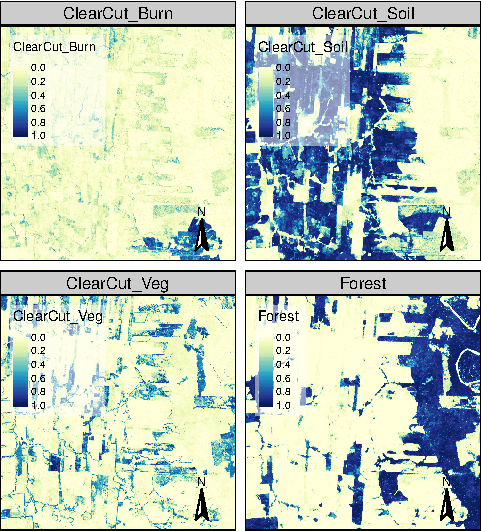
\includegraphics{Bayesian_smoothing_JSS_files/figure-latex/pcube-1} 

}

\caption[Class probabilities produced by random forest algorithm]{Class probabilities produced by random forest algorithm}\label{fig:pcube}
\end{figure}
\end{CodeChunk}

Figure \ref{fig:pcube} shows the plot of the probability images for classes \code{Forest}, \code{ClearCut_Soil}, \code{ClearCut_Veg} and \code{ClearCut_Burn}. The map for class \code{Forest} shows high probability values associated with compact patches. Class \code{ClearCut_Soil} is mostly composed of dense areas of high probability whose geometrical boundaries result from forest cuts. The class \code{ClearCut_Veg} is less well-defined than the others; this is to be expected since this is a transitional class between a natural forest and areas of bare soil. Patches associated to class \code{ClearCut_Burn} include both homogeneous areas of high probability and areas of mixed response. Since classes have different behaviours, the post-processing procedure should enable users to control how to handle outliers and border pixels of each class.

The next step is to show the labelled map resulting from the raw class probabilites. Figure \ref{fig:map1} shows the classification map, obtained by taking the class of higher probability to each pixel, without considering the spatial context. There are many places with the so-called ``salt-and-pepper'' effect which result from misclassified pixels. The non-smoothed labelled map shows the need for post-processing, since it contains a significant number of outliers and areas with mixed labelling.

\begin{CodeChunk}
\begin{CodeInput}
R> # produce a labelled map
R> map_no_smooth <- bayes_label(probs_image)
R> # show the map
R> bayes_plot_map(map_no_smooth)
\end{CodeInput}
\begin{figure}[h]

{\centering 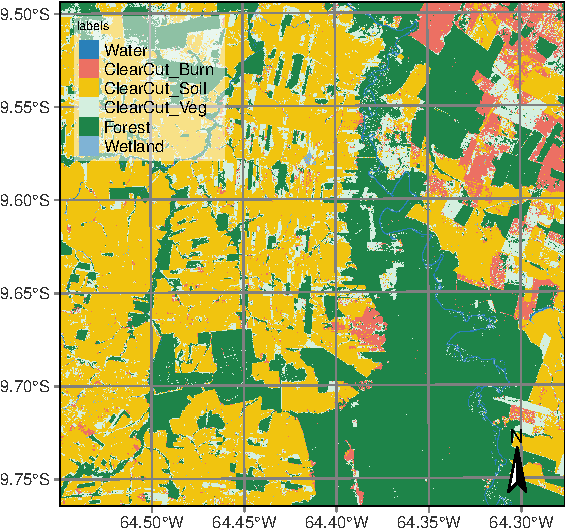
\includegraphics{Bayesian_smoothing_JSS_files/figure-latex/map1-1} 

}

\caption[Labelled map without smoothing]{Labelled map without smoothing.}\label{fig:map1}
\end{figure}
\end{CodeChunk}

\subsection{Estimating the local logit variances}\label{estimating-the-local-logit-variances}

The local logit variances correspond to the \(s^2_{i,k}\) parameter in the Bayesian inference and are estimated by \code{bayes_variance()}. Its main parameters are: (a) a \code{SpatRaster} object ; (b) \code{window_size}, dimension of the local neighbourhood; (c) \code{neigh_fraction}, the percentage of pixels in the neighbourhood used to calculate the variance. The example below uses half of the pixels of a \(7\times 7\) window to estimate the variance. The chosen pixels will be those with the highest probability pixels to be more representative of the actual class distribution. The output values are the logit variances in the vicinity of each pixel.

\begin{CodeChunk}
\begin{CodeInput}
R> var_image <- bayes_variance(
+     x = probs_image,
+     window_size = 7,
+     neigh_fraction = 0.50)
R> bayes_summary(var_image)
\end{CodeInput}
\begin{CodeOutput}
 Water             ClearCut_Burn       ClearCut_Soil       ClearCut_Veg     
 Min.   : 0.0000   Min.   : 0.002481   Min.   : 0.003603   Min.   : 0.0000  
 1st Qu.: 0.2017   1st Qu.: 0.072208   1st Qu.: 0.100210   1st Qu.: 0.1116  
 Median : 2.3265   Median : 0.150143   Median : 0.225121   Median : 0.2836  
 Mean   : 2.6266   Mean   : 0.331228   Mean   : 0.614570   Mean   : 0.6481  
 3rd Qu.: 4.7932   3rd Qu.: 0.310010   3rd Qu.: 0.550980   3rd Qu.: 0.7507  
 Max.   :21.7559   Max.   :11.260116   Max.   :10.368152   Max.   :16.8963  
 Forest            Wetland           
 Min.   : 0.0000   Min.   : 0.00000  
 1st Qu.: 0.1159   1st Qu.: 0.07297  
 Median : 0.4922   Median : 0.16622  
 Mean   : 1.6533   Mean   : 0.49490  
 3rd Qu.: 2.5643   3rd Qu.: 0.35359  
 Max.   :23.2210   Max.   :10.39689  
\end{CodeOutput}
\end{CodeChunk}

The choice of the \(7 \times 7\) window size is a compromise between having enough values to estimate the parameters of a normal distribution and the need to capture local effects for class patches of small sizes. Classes such as \code{Water} and \code{ClearCut_Burn} tend to be spatially limited; a bigger window size could result in invalid values for their respective normal distributions.

The summary statistics show that most local variance values are low, which is an expected result. Areas of low variance correspond to pixel neighborhoods of high logit values for one of the classes and low logit values for the others. High values of the local variances are relevant in areas of confusion between classes. Figure \ref{fig:vcube} shows the values of local logit variances for classes \code{ClearCut_Soil}, \code{ClearCut_Burn}, \code{ClearCut_Veg}, and \code{Forest}. Only the top 25\% of the values for each class are shown, emphasizing areas of high local variability.

\begin{CodeChunk}
\begin{CodeInput}
R> bayes_plot_var(var_image, 
+                  quantile = 0.75, 
+                  palette = "Greens",
+                  labels = c("ClearCut_Soil", "Forest"))
\end{CodeInput}
\begin{figure}[h]

{\centering 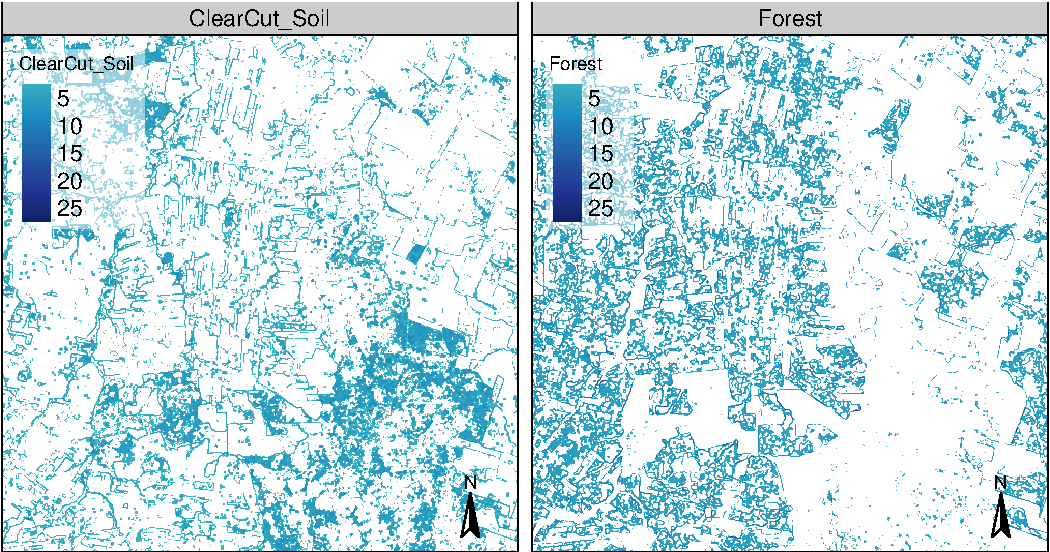
\includegraphics{Bayesian_smoothing_JSS_files/figure-latex/vcube-1} 

}

\caption[Logit variance map showing values above the 3rd quartile for classes ClearCutSoil and Forest]{Logit variance map showing values above the 3rd quartile for classes ClearCutSoil and Forest.}\label{fig:vcube}
\end{figure}
\end{CodeChunk}

\begin{CodeChunk}
\begin{CodeInput}
R> bayes_plot_var(var_image, 
+                  quantile = 0.75, 
+                  palette = "Greens",
+                  labels = c("ClearCut_Veg", "ClearCut_Burn"))
\end{CodeInput}
\begin{figure}[h]

{\centering 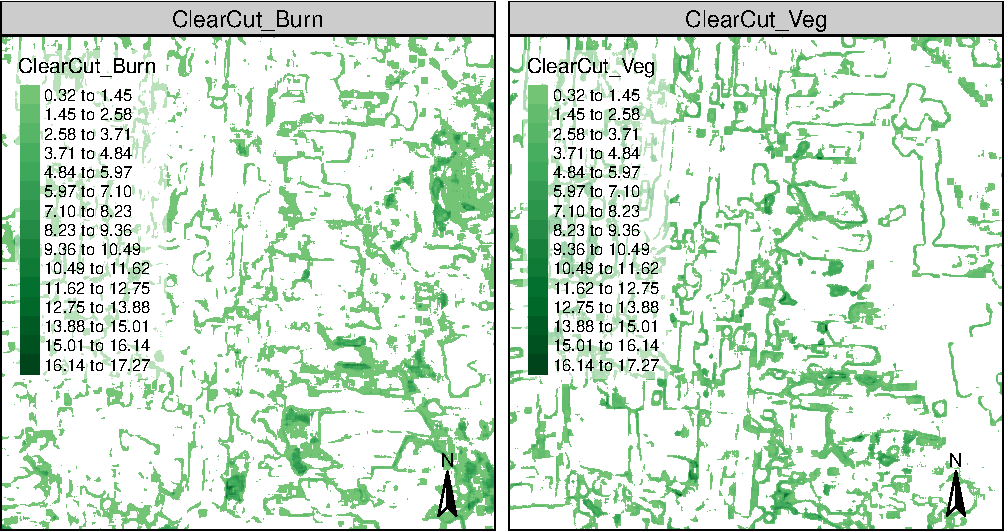
\includegraphics{Bayesian_smoothing_JSS_files/figure-latex/vcuben-1} 

}

\caption[Logit variance map showing values above the 3rd quartile for classes ClearCutVeg and ClearCutBurn]{Logit variance map showing values above the 3rd quartile for classes ClearCutVeg and ClearCutBurn.}\label{fig:vcuben}
\end{figure}
\end{CodeChunk}

\FloatBarrier

Comparing the variance maps of Figure \ref{fig:vcube} with the probability maps of Figure \ref{fig:pcube}, one sees that areas of high probability of classes \code{Forest} and \code{ClearCut_Soil} are mostly made of compact patches. Recall these are the two dominant classes in the area, and deforestation is a process that converts forest to bare soil. Many areas of high logit variance for these classes are related to border pixels which have a mixed response. Areas of large patches of high logit variance for these classes are associated to lower class probabilities and will not be relevant to the final result.

By contrast, the transitional classes \code{ClearCut_Veg} and \code{ClearCut_Burn} have a different spatial pattern of their probability and logit variance. Class \code{ClearCut_Veg} has a high spatial variability, since pixels of this class arise when the forest has not been completely removed and there is some remaining vegetation after trees are cut. The extent of remaining vegetation after most trees have been removed is not uniform. For this reason, many areas of high local logit variance of class \code{ClearCut_Veg} are located in mixed patches inside pixels of class \code{Forest}.

Instances of class \code{ClearCut_Burn} arise following a forest fire. As shown in Figure \ref{fig:pcube}, most pixels of this class tend to form mid-sized to large spatial clusters, because of how forest fires start and propagate. It is desirable to preserve the contiguity of the burned areas and remove pixels of other classes inside these clusters. Isolated points of class \code{ClearCut_Burn} can be removed without significant information loss.

What emerges from the above analysis is that each land cover and land use class has different expected spatial patters. For this reason, it is useful to use the variance data to support adequate assigment of \(\sigma^2_k\) value. We compute the top 25\% of the logit variance values and use them for an informed choice of the hyperparameter.

\begin{CodeChunk}
\begin{CodeInput}
R> # function to return quantiles for the logit variances
R> var_quantiles <- function(var_image, intervals, quantiles){
+   values <- terra::spatSample(var_image, size = 15000, na.rm = TRUE)
+   mat <- apply(values, 2, function(x){ 
+     quantile(x, probs = seq(0, 1, intervals))
+   })
+   return(mat[quantiles, ])
+ }
R> # get the 75%-95% quantiles
R> var_quantiles(var_image, 0.05, c("75%", "80%", "85%", "90%", "95%", "100%"))
\end{CodeInput}
\begin{CodeOutput}
         Water ClearCut_Burn ClearCut_Soil ClearCut_Veg    Forest    Wetland
75%   4.764197     0.3147544     0.5568953    0.7583870  2.662210  0.3547823
80%   4.971079     0.3789011     0.7222972    0.9521859  3.433133  0.4273479
85%   5.148950     0.4670305     1.0232807    1.2087787  4.324530  0.5382029
90%   5.422300     0.6047362     1.5498801    1.6012467  5.040908  0.7697119
95%   6.016208     0.9556933     2.8438386    2.3973728  5.835870  2.3830680
100% 24.353707    12.8347503    14.2305099   14.4590720 21.898716 11.3679790
\end{CodeOutput}
\end{CodeChunk}

\subsection{Applying Bayesian smoothing to remove outliers}\label{applying-bayesian-smoothing-to-remove-outliers}

To remove the outliers, \pkg{bayesEO} provides \code{bayes_smooth()}. Its main parameters are: (a) \code{x}, a probability image; (b) \code{window_size}, dimension of the local neighbourhood; (c) \code{smoothness}, values of \(\sigma^2_{k}\) for each class. The impact of Bayesian smoothing can be best captured by producing a labelled map using \code{bayes_label()}, taking the smoothed image as its input.

We choose values of \(\sigma^2_{k}\) that reflect our prior expectation of the spatial patterns of each class. For classes \code{ClearCut_Veg} and \code{ClearCut_Burn}, to produce denser spatial clusters and remove ``salt-and-pepper'' outliers, we take \(\sigma^2_{k}\) values in 95\%-100\% range. In the case of the most frequent classes \code{Forest} and \code{ClearCut_Soil} we want to preserve their original spatial shapes as much as possible; the same logic applies to less frequent classes \code{Water} and \code{Wetlands}. For this reason, we set \(\sigma^2_{k}\) values in the 75\%-80\% range for these classes. Figure \ref{fig:smth1} shows that the outliers and isolated pixels have been removed. The class spatial patterns correspond to our prior expectations.

\begin{CodeChunk}
\begin{CodeInput}
R> map_smooth_bayes <- bayes_smooth(probs_image,
+     window_size = 7,
+     smoothness = c( "Water" = 5.0, "ClearCut_Burn" = 20, "ClearCut_Soil" = 1, 
+       "ClearCut_Veg" =  15, "Forest" = 3.5, "Wetland" = 0.40)
+     ) |> bayes_label()
R> bayes_plot_map(map_smooth_bayes)
\end{CodeInput}
\begin{figure}[h]

{\centering 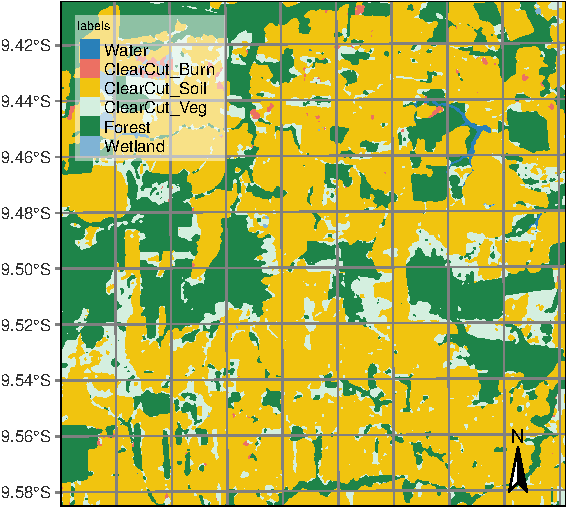
\includegraphics{Bayesian_smoothing_JSS_files/figure-latex/smth1-1} 

}

\caption[Labeled map with Bayesian  smoothing]{Labeled map with Bayesian  smoothing.}\label{fig:smth1}
\end{figure}
\end{CodeChunk}

\FloatBarrier

In the smoothed map (Figure \ref{fig:smth1}), the most frequent classes (\code{ClearCut_Soil} and \code{Forest}) increased slightly their areas at the expense of the others. The class \code{ClearCut_Burn} now appear as dense patches as befits areas affected by forest fire, while class \code{ClearCut_Veg} has preserved most of their areas, while removing outliers.

\newpage

\section{Comparison with other methods}\label{comparison-with-other-methods}

To better understand the benefits of Bayesian smoothing, we present the results of post-processing using two alternatives: Gaussian smoothing and bilateral smoothing. Gaussian smoothing is a low-pass filter where the weights are based on the normal distribution. Pixels near the center of the kernel have a higher weight, and the weight decreases for pixels further away from the center. This creates a blurring effect that is stronger at the center and weaker at the edges.

\begin{equation}
   I'(x, y) = \sum_{i=-k}^{k} \sum_{j=-k}^{k} \frac{1}{2\pi\sigma^2} e^{-\frac{(x-i)^2 + (y-j)^2}{2\sigma^2}} \cdot I(x - i, y - j)
\end{equation}

In this equation, \(I'(x, y)\) represents the smoothed image, \(I(x, y)\) is the original image, \((i,j)\) are the indices running over the kernel size, and where \(\sigma\) is the standard deviation a Gaussian distribution.

The following code computes a Gaussian filter, labels the image and plots the resulting map.

\begin{CodeChunk}
\begin{CodeInput}
R> # compute Gaussian smoothing, label and plot map
R> map_gaussian <- gaussian_smooth(probs_image, window_size = 7, sigma = 5 ) |> 
+   bayes_label()
R> bayes_plot_map(map_gaussian)
\end{CodeInput}
\begin{figure}[h]

{\centering 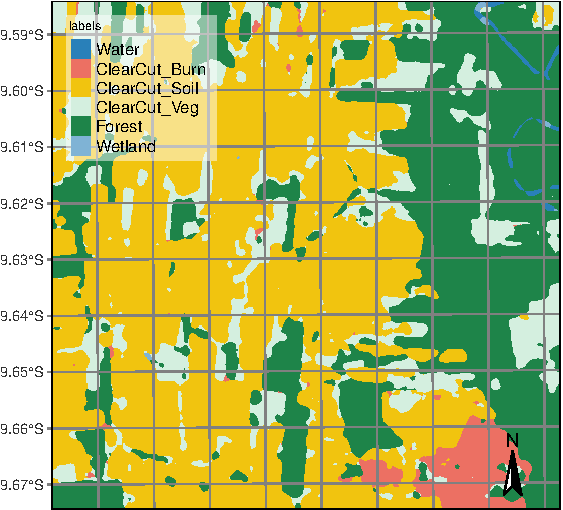
\includegraphics{Bayesian_smoothing_JSS_files/figure-latex/gauss-1} 

}

\caption[Labeled map using Gaussian smoothing]{Labeled map using Gaussian smoothing.}\label{fig:gauss}
\end{figure}
\end{CodeChunk}

Comparison between Figure \ref{fig:smth1} and Figure \ref{fig:gauss} shows subtle but important differences. Bayesian smoothing does a better job of preserving edges and small homogeneous areas than Gaussian filtering. The result is a more consistent map. Parameters for Gaussian smoothing are the same for each class and assume isotropic neighbourhoods, while Bayesian inference allows the expert to control the output for each class. Moreover, the parameter \(\sigma\) for Gaussian filtering was set by trial-and-error. The above example shows the best result after trying different alternatives.

Bilateral smoothing aims to reduce noise while preserving edges. Unlike the Gaussian filter, which can blur edges, the bilateral filter maintains sharp edges by taking into account the difference in intensity values between pixels \citep{Tomasi1998}. Bilateral filtering combines a spatial filter, like the Gaussian filter, which considers the spatial closeness of pixels, with a range filter, which considers the similarity in intensity values between pixels. By considering intensity differences, the bilateral filter can preserve edges.

The bilateral filter has two main parameters: (a) the spatial parameter \(\sigma\) controls the spatial extent of the kernel; (b) the range parameter \(\tau\) controls how much a pixel must differ in intensity for it to be considered different. Its mathematical expression is

\begin{equation}
I'(x, y) = \frac{1}{W(x, y)} \sum_{i=-k}^{k} \sum_{j=-k}^{k} I(x - i, y - j) \cdot G_{\sigma}(i, j) \cdot G_{\tau}(I(x - i, y - j) - I(x, y))
\end{equation}

where \(I'(x,y)\) is the filtered image and \(I(x,y)\) is the original image. \(G_{\sigma}(i, j)\) is the spatial Gaussian function, which decreases with distance from the central pixel, controlled by the spatial standard deviation \(\sigma\). \(G_{\tau}(I(x + i, y + j) - I(x, y))\) is the range Gaussian function, which decreases with the intensity difference between the neighboring pixel and the central pixel controlled by the range standard deviation \(\tau\).

\(W(x, y)\) is a normalization factor defined as
\begin{equation}
W(x, y) = \sum_{i=-k}^{k} \sum_{j=-k}^{k} G_{\sigma_s}(i, j) \cdot G_{\sigma_r}(I(x - i, y - j) - I(x, y))
\end{equation}

This formula illustrates how the bilateral filter considers both spatial proximity and intensity similarity in its smoothing process, thereby preserving edges while reducing noise in other areas. The following code performs bilateral smoothing.

\begin{CodeChunk}
\begin{CodeInput}
R> # compute Bilateral smoothing
R> bilat_smooth <- bilateral_smooth(
+     probs_image,
+     window_size = 7,
+     sigma = 5,
+     tau = 2.0
+ )
R> # produce the labelled map
R> map_bilat <- bayes_label(bilat_smooth)
R> # plot the map produced by Bilateral smoothing
R> bayes_plot_map(map_bilat)
\end{CodeInput}
\begin{figure}[h]

{\centering 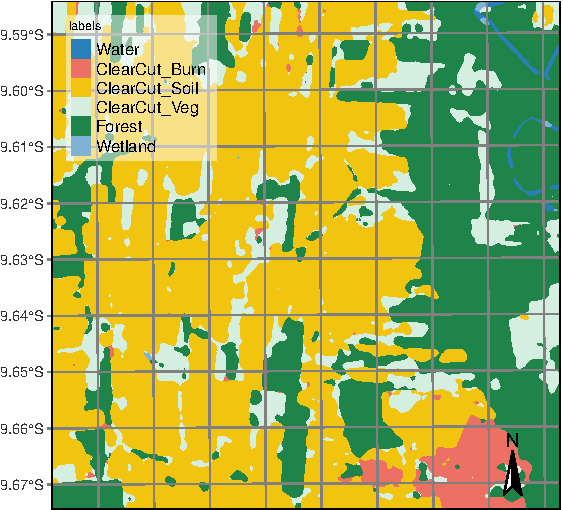
\includegraphics{Bayesian_smoothing_JSS_files/figure-latex/bilat-1} 

}

\caption[Labeled map using bilateral smoothing]{Labeled map using bilateral smoothing.}\label{fig:bilat}
\end{figure}
\end{CodeChunk}

The resulting map after bilateral smoothing is similar to the output of Bayesian smoothing. However, this result required some rounds of trial and error to set the best values for the \(\sigma\) and \(\tau\) parameters. There is no objective method for choosing the appropriate values for them. By contrast, the smoothness parameters for Bayesian filtering are based on expert knowledge. To better assert the impact of smoothing, consider the class areas in the non-smoothed and smoothed maps and compare with the results of gaussian and bilateral filters.

\begin{CodeChunk}
\begin{CodeInput}
R> # get the summary of the non-smoothed map
R> sum1 <- bayes_summary(map_no_smooth)
R> colnames(sum1) <- c("class", "no_smooth")
R> # get the summary of the smoothed map
R> sum2 <- bayes_summary(map_smooth_bayes)
R> colnames(sum2) <- c("class", "smooth")
R> # get the summary of the gaussian map
R> sum3 <- bayes_summary(map_gaussian)
R> colnames(sum3) <- c("class", "gauss")
R> # get the summary of the bilateral map
R> sum4 <- bayes_summary(map_bilat)
R> colnames(sum4) <- c("class", "bilat")
R> # compare class areas of non-smoothed and smoothed maps
R> dplyr::inner_join(sum1, sum2, by = "class") |> 
+   dplyr::inner_join(sum3, by = "class") |> 
+   dplyr::inner_join(sum4, by = "class") 
\end{CodeInput}
\begin{CodeOutput}
# A tibble: 6 x 5
  class         no_smooth smooth  gauss  bilat
  <chr>             <dbl>  <dbl>  <dbl>  <dbl>
1 Water              0.51   0.46  0.38   0.4  
2 ClearCut_Burn      4.59   3.19  3.08   3.08 
3 ClearCut_Soil     47.2   48.9  51.0   50.9  
4 ClearCut_Veg      17.1   16.0  14.1   14.2  
5 Forest            30.2   31.3  31.4   31.3  
6 Wetland            0.38   0.13  0.087  0.088
\end{CodeOutput}
\end{CodeChunk}

Bayesian smoothing does a better job at preserving the original class areas, while producing compact shapes and removing outliers. While the area differences in this example are relatively small, they tend to increase in large regions with multiple classes. This example shows the value of the Bayesian inference procedure compared with Gaussian and bilateral filtering. Most post-classification procedures use ad-hoc parameters which are not directly linked to the properties of the data. These parameters are based on the structure of the algorithm (e.g, size of the Gaussian kernel), not being easily defined separately for each class. Bayesian inference allows the expert to control the output and to set the parameters based on objective criteria.

\section{Using smoothing in connection with time-first, space-later methods}\label{using-smoothing-in-connection-with-time-first-space-later-methods}

Time-first, space-later is a concept in satellite image classification that takes time series analysis as the first step for analysing remote sensing data, with spatial information being considered after all time series are classified \citep{Camara2016}. Satellite image time series are calibrated and comparable measures of the same location on Earth at different times. When associated with frequent revisits, image time series can capture significant land use and land cover changes. Detecting and tracking seasonal and long-term trends becomes feasible, as well as identifying anomalous events or patterns in the data, such as wildfires, floods, or droughts \citep{Woodcock2020}.

This approach takes image time series as the first step for analysing remote sensing data. The \textit{time-first} part brings a better understanding of changes in landscapes. Detecting and tracking seasonal and long-term trends becomes feasible, as well as identifying anomalous events or patterns in the data, such as wildfires, floods, or droughts. Each pixel in a data cube is treated as a time series, using information available in the temporal instances of the case. Time series classification is pixel-based, producing a set of labeled pixels. This result is then used as input to the \textit{space-later} part of the method. In this phase, Bayesian algorithm improves the results of time-first classification by considering the spatial neighbourhood of each pixel. The resulting map thus combines both spatial and temporal information. Recent reviews of deep learning classification using image time series highlight the value of post-classification spatial smoothing \citep{Perbet2024}. Thus, Bayesian smoothing is an important component of the time-first, space-later Earth observation data analysis.

The Bayesian smoothing method proposed in the paper has proven valuable in a number of studies that use the \proglang{R} \pkg{sits} for land use classification of image time series \citep{Picoli2018, Simoes2020, Hadi2023, Giuliani2024, Werner2024}. The availability of the method as a stand-alone \pkg{bayesEO} is intended to broaden the target user community and make it easier for \proglang{R} experts to combine the algorithm in their scripts.

\section{Conclusion}\label{conclusion}

This paper presents a new method for post-processing of Earth observation images that have been classified using machine learning algorithms. Unlike ad-hoc smoothing methods avaliable in the literature, the proposed algorithm relies on objective metrics of class probability variance. We propose an Empirical Bayes approach to post-processing, which has a sound mathematical basis. The method has been validated for large-scale data analysis in connection with a time-first, space-based approach and represents a worthy alternative to other post-processing methods available in the literature.

\subsection*{Acknowledgments}\label{acknowledgments}
\addcontentsline{toc}{subsection}{Acknowledgments}

The authors acknowledge the support of the following institutions: (a) Amazon Fund, established by Brazil with financial contribution from Norway, through contract 17.2.0536.1.; (b) International Climate Initiative of the Germany Federal Ministry for the Environment, Nature Conservation, Building and Nuclear Safety (IKI) under grant 17-III-084-Global-A-RESTORE+ (``RESTORE+: Addressing Landscape Restoration on Degraded Land in Indonesia and Brazil''); (c) Microsoft Planetary Computer initiative under the GEO-Microsoft Cloud Computer Grants Programme; (d) Instituto Clima e Sociedade, under the project grant ``Modernization of PRODES and DETER Amazon monitoring systems'' (grants G-22-01193 and G-23-01643); (e) Open-Earth-Monitor Cyberinfrastructure project, under European Commission grant agreement No.~101059548.

\bibliography{e-sensing.bib}



\end{document}
